% Figure 1: the same sentence read as bytes, as BPE tokens, and as H-Net chunks.
% Token cuts come from our 32k BPE tokenizer; chunk cuts come from the trained
% H-Net (chunk_viz.py on runs/hnet-44B).
\documentclass[tikz,border=10pt]{standalone}
\usepackage[T1]{fontenc}
\usepackage[scaled=0.92]{helvet}
\renewcommand{\familydefault}{\sfdefault}

\definecolor{ink}{HTML}{1F1F1E}
\definecolor{quiet}{HTML}{6B6A66}
\definecolor{accent}{HTML}{2A78D6}
\definecolor{accentsoft}{HTML}{E4EEFB}
\definecolor{warm}{HTML}{B8742A}
\definecolor{warmsoft}{HTML}{FAEEDD}
\definecolor{greysoft}{HTML}{EFEEEA}
\definecolor{greyline}{HTML}{A8A69E}

% one character cell is \cw cm wide
\newcommand{\cw}{0.38}
% a visible space
\newcommand{\vsp}{\textcolor{quiet}{\textbullet}}
% the sentence, one entry per byte (35 bytes)
\newcommand{\sentence}{T,h,e,\vsp,F,r,e,n,c,h,\vsp,R,e,v,o,l,u,t,i,o,n,\vsp,b,e,g,a,n,\vsp,i,n,\vsp,1,7,8,9}

% \chunkrow{y}{list of chunk lengths}{box style}
% draws one box per chunk, then the characters on top
\newcommand{\chunkrow}[3]{%
  \gdef\xoff{0}%
  \foreach \n in {#2} {%
    \draw[rounded corners=2.5pt, line width=0.7pt, #3]
      ({\xoff*\cw+0.035}, {#1-0.30}) rectangle ({(\xoff+\n)*\cw-0.035}, {#1+0.30});
    \pgfmathtruncatemacro{\next}{\xoff+\n}%
    \xdef\xoff{\next}%
  }%
  \foreach \c [count=\i from 0] in \sentence {%
    \node[text=ink, font=\ttfamily\small, inner sep=0pt] at ({(\i+0.5)*\cw}, {#1}) {\strut\c};
  }%
}

\begin{document}
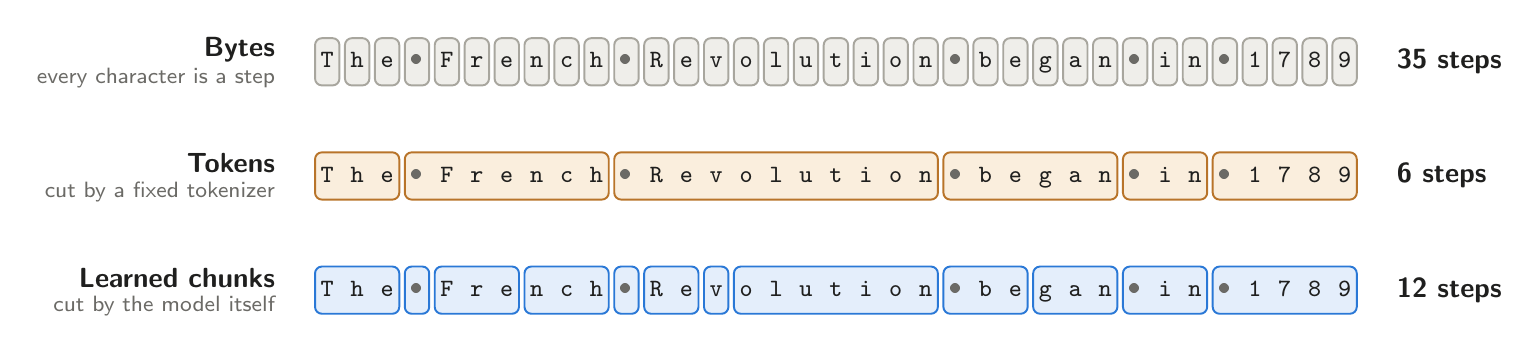
\begin{tikzpicture}[
    label/.style={anchor=east, text=ink, font=\bfseries, align=right},
    sub/.style={anchor=east, text=quiet, font=\footnotesize, align=right},
    count/.style={anchor=west, text=ink, font=\bfseries},
  ]
  \pgfmathsetmacro{\rowend}{35*\cw}

  % row 1: bytes
  \chunkrow{0}{1,1,1,1,1,1,1,1,1,1,1,1,1,1,1,1,1,1,1,1,1,1,1,1,1,1,1,1,1,1,1,1,1,1,1}{draw=greyline, fill=greysoft}
  \node[label] at (-0.35, 0.16) {Bytes};
  \node[sub]   at (-0.35,-0.20) {every character is a step};
  \node[count] at (\rowend+0.35, 0) {35 steps};

  % row 2: BPE tokens  The | French | Revolution | began | in | 1789
  \chunkrow{-1.45}{3,7,11,6,3,5}{draw=warm, fill=warmsoft}
  \node[label] at (-0.35,-1.29) {Tokens};
  \node[sub]   at (-0.35,-1.65) {cut by a fixed tokenizer};
  \node[count] at (\rowend+0.35,-1.45) {6 steps};

  % row 3: H-Net chunks  The| |Fre|nch| |Re|v|olution| be|gan| in| 1789
  \chunkrow{-2.90}{3,1,3,3,1,2,1,7,3,3,3,5}{draw=accent, fill=accentsoft}
  \node[label] at (-0.35,-2.74) {Learned chunks};
  \node[sub]   at (-0.35,-3.10) {cut by the model itself};
  \node[count] at (\rowend+0.35,-2.90) {12 steps};
\end{tikzpicture}
\end{document}
